\chapter{Introduction}
\label{chapter-1}
\vfill
\begin{center}
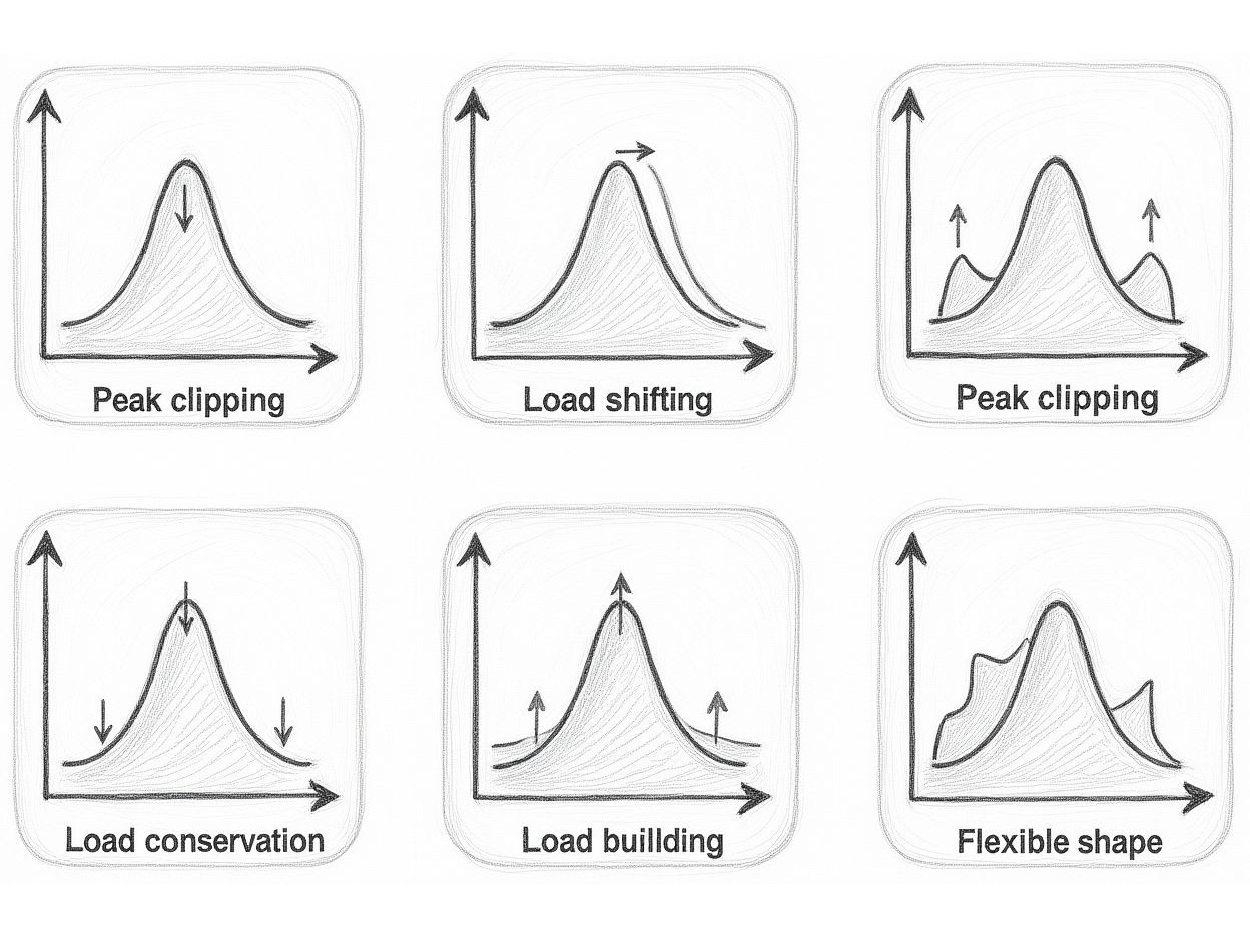
\includegraphics[width=\textwidth]{figures/chapter_1/type_flex_sketch.pdf}
\end{center}
\newpage
% These can be used to do keywords
\section{Different design for putting keywords}
\subsection{One row}
\noindent
K\ E\ Y\ W\ O\ R \ D\ S

\noindent
\keywordtag{Congestion} \hfill
\keywordtag{Flexibility} \hfill
\keywordtag{Smart Charging} \hfill
\keywordtag{Market Product}

\vspace{1 em}
\noindent
\subsection{Multiple row with vertical heading}

\begin{minipage}[b]{0.075\linewidth} 
  \rotatebox[origin=l]{90}{K\ E\ Y\ W\ O\ R \ D\ S \rule{2cm}{0.4pt}} 
\end{minipage}%
\begin{minipage}[b]{0.9\linewidth} % 65% width
\keywordtag{Aggregate Charging}\\
\vspace{0.5 pt}\\
\keywordtag{Congestion} \\
\vspace{0.5 pt}\\
\keywordtag{Electric Vehicles}\\
\vspace{0.5 pt}\\
\keywordtag{Flexibility} \\
\vspace{0.5 pt}\\
\keywordtag{Smart Charging} \\
\end{minipage}
\subsection{Multiple row with horizontal heading}
K\ E\ Y\ W\ O\ R \ D\ S \hrulefill

\noindent
\keywordtag{Aggregate Charging}\\
\vspace{0.5 pt}\\
\keywordtag{Congestion} \\
\vspace{0.5 pt}\\
\keywordtag{Electric Vehicles}\\
\vspace{0.5 pt}\\
\keywordtag{Flexibility} \\
\vspace{0.5 pt}\\
\newpage
\section{Chapter summary style}
\subsection{Horizontal heading}

O\ V\ E\ R\ V\ I\ E\ W \hrulefill\\
\lettrine{\color{royal_blue}E}{nergy} i\lipsum[5]
\subsection{Vertical heading}
\begin{minipage}[b]{0.075\linewidth} 
  \rotatebox[origin=l]{90}{O\ V\ E\ R\ V\ I\ E\ W \rule{2cm}{0.4pt}} 
\end{minipage}%
\begin{minipage}[b]{0.9\linewidth} % 65% width
\lettrine{\color{royal_blue}E}{nergy} \lipsum[8]
\end{minipage}

 

 \vfill
\rule{\textwidth}{0.4pt}
Here you can use this space to refer to the publication on which the following chapter is based. For example, the contents of this chapter are related to the publication: Panda, N. K., \& Tindemans, S. H. (2024). \textit{Quantifying the Aggregate Flexibility of Electric Vehicles Charging Stations for Dependable Congestion Management Products - A Dutch Case Study. \textit{arXiv preprint} \href{https://arxiv.org/abs/2403.13367}{arXiv:2403.13367}.}
\newpage
\section{Using abbreviations}
To streamline the use of abbreviations, it is recommended to use the \say{acronym} package. Then you can write abbreviations like \ac{EV} by defining at a single point as inside the acronym\_list.tex under frontmatter. Plural form of the abbreviation can be written as \acp{EV}, and the full form can be called as \acf{EV}.
\section{Using text box}
To highlight a certain concept, you can use a text box, such as:
\begin{tcolorbox}[colback=delft_blue_shade2,colframe=delft_blue_shade1,title=\textbf{Congestion}]
\begin{wrapfigure}{r}{0.3\linewidth}
    \centering
    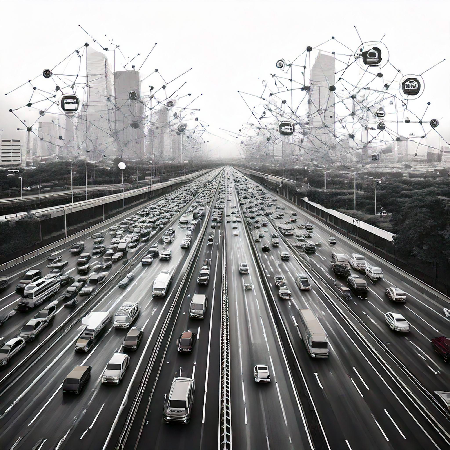
\includegraphics[width=1\linewidth]{figures/chapter_1/congestion_clip_art.pdf}
\end{wrapfigure}
\lipsum[8]
\end{tcolorbox}
\section{Using reference}
Things can be cited like \cite{panda2024aggregate}. Then it will automatically be shown in the Bibliography, provided a supporting \say{.bib} file is supplied. Make sure not to have duplicate entries in the file. 
\section{Section 4}
\lipsum[5]
